\documentclass[border=10pt]{standalone}
\usepackage{tikz}
\usetikzlibrary{shapes.geometric, arrows.meta, positioning, fit, calc, backgrounds, shadows}

\begin{document}
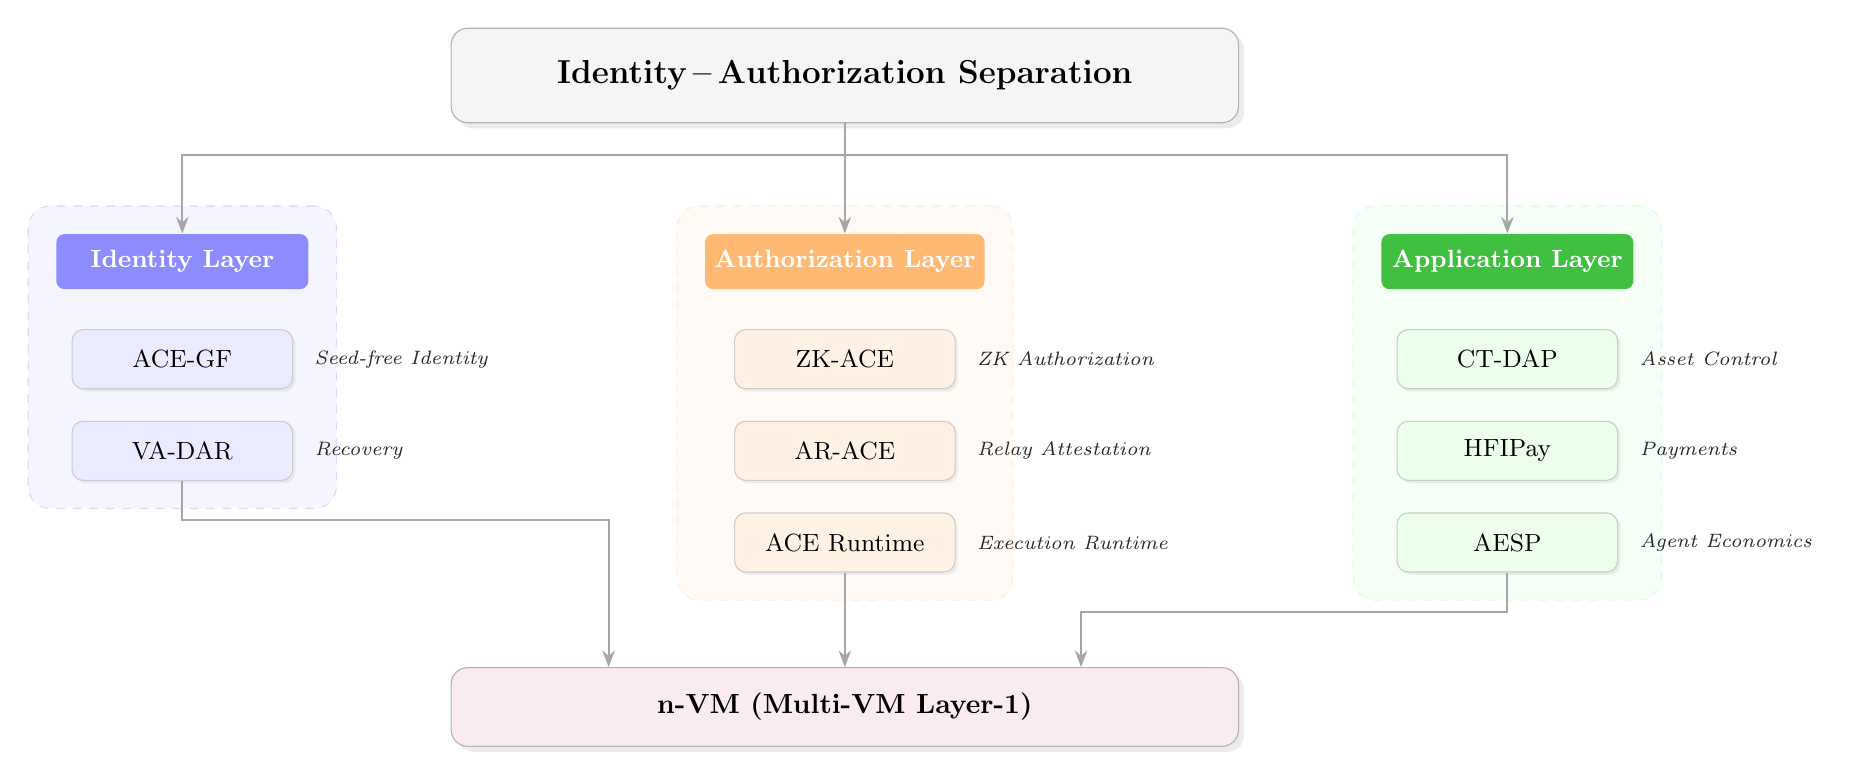
\begin{tikzpicture}[
    node distance=0.8cm and 1.2cm,
    font=\sffamily,
    every node/.style={align=center},
    arrow/.style={-{Stealth[length=6pt]}, thick, color=gray!70},
]

% --- Style definitions ---
\tikzset{
    principle/.style = {draw=gray!60, rounded corners=6pt, fill=gray!8,
        minimum height=1.2cm, minimum width=10cm, align=center, font=\large\bfseries, text=black,
        drop shadow={opacity=0.15, shadow xshift=2pt, shadow yshift=-2pt}},
    layertitle/.style = {font=\small\bfseries, text=white, minimum height=0.7cm,
        minimum width=3.2cm, rounded corners=3pt},
    component/.style = {draw=gray!40, rounded corners=4pt, minimum height=0.75cm,
        minimum width=2.8cm, font=\small, text=black,
        drop shadow={opacity=0.12, shadow xshift=1pt, shadow yshift=-1pt}},
    identity/.style = {component, fill=blue!8},
    authz/.style = {component, fill=orange!10},
    app/.style = {component, fill=green!8},
    integration/.style = {draw=gray!60, rounded corners=6pt, fill=purple!8,
        minimum height=1.0cm, minimum width=10cm, font=\bfseries, text=black,
        drop shadow={opacity=0.15, shadow xshift=2pt, shadow yshift=-2pt}},
    lbl/.style = {font=\scriptsize, text=black!85},
}

% --- Top: Principle ---
\node (principle) [principle] {Identity\,--\,Authorization Separation};

% --- Layer titles ---
\node (id-title) [layertitle, fill=blue!45, below left=1.4cm and 1.8cm of principle] {Identity Layer};
\node (auth-title) [layertitle, fill=orange!55, below=1.4cm of principle] {Authorization Layer};
\node (app-title) [layertitle, fill=green!50!gray, below right=1.4cm and 1.8cm of principle] {Application Layer};

% --- Identity Layer components ---
\node (acegf) [identity, below=0.5cm of id-title] {ACE-GF};
\node (vadar) [identity, below=0.4cm of acegf] {VA-DAR};

% --- Authorization Layer components ---
\node (zkace) [authz, below=0.5cm of auth-title] {ZK-ACE};
\node (arace) [authz, below=0.4cm of zkace] {AR-ACE};
\node (aceruntime) [authz, below=0.4cm of arace] {ACE Runtime};

% --- Application Layer components ---
\node (ctdap) [app, below=0.5cm of app-title] {CT-DAP};
\node (hfipay) [app, below=0.4cm of ctdap] {HFIPay};
\node (aesp) [app, below=0.4cm of hfipay] {AESP};

% --- Component descriptions (right-aligned labels) ---
\node [lbl, right=0.15cm of acegf] {\textit{Seed-free Identity}};
\node [lbl, right=0.15cm of vadar] {\textit{Recovery}};
\node [lbl, right=0.15cm of zkace] {\textit{ZK Authorization}};
\node [lbl, right=0.15cm of arace] {\textit{Relay Attestation}};
\node [lbl, right=0.15cm of aceruntime] {\textit{Execution Runtime}};
\node [lbl, right=0.15cm of ctdap] {\textit{Asset Control}};
\node [lbl, right=0.15cm of hfipay] {\textit{Payments}};
\node [lbl, right=0.15cm of aesp] {\textit{Agent Economics}};

% --- Arrows from principle to layer titles ---
\draw [arrow] (principle.south) -- ++(0, -0.4) -| (id-title.north);
\draw [arrow] (principle.south) -- (auth-title.north);
\draw [arrow] (principle.south) -- ++(0, -0.4) -| (app-title.north);

% --- Bottom: n-VM Integration (centered under the full diagram) ---
\node (nvm) [integration, below=1.2cm of aceruntime, xshift=0cm] {n-VM (Multi-VM Layer-1)};

% --- Arrows to n-VM ---
\draw [arrow] (vadar.south) -- ++(0, -0.5) -| ([xshift=-3cm]nvm.north);
\draw [arrow] (aceruntime.south) -- (nvm.north);
\draw [arrow] (aesp.south) -- ++(0, -0.5) -| ([xshift=3cm]nvm.north);

% --- Background grouping ---
\begin{scope}[on background layer]
    \node [fit=(id-title)(acegf)(vadar), fill=blue!4, rounded corners=8pt,
        draw=blue!15, dashed, inner sep=0.35cm] {};
    \node [fit=(auth-title)(zkace)(arace)(aceruntime), fill=orange!4, rounded corners=8pt,
        draw=orange!15, dashed, inner sep=0.35cm] {};
    \node [fit=(app-title)(ctdap)(hfipay)(aesp), fill=green!4, rounded corners=8pt,
        draw=green!15, dashed, inner sep=0.35cm] {};
\end{scope}

\end{tikzpicture}
\end{document}
